%beamer

% Comment/uncomment this line to toggle handout mode
\newcommand{\handout}{}

%% Beamer-Klasse im korrekten Modus
\ifdefined \handout
\documentclass[handout]{beamer} % Handout mode
\else
\documentclass{beamer}
\fi

%% UTF-8-Encoding
\usepackage[utf8]{inputenc}

\input{../framework/gbi-macros}
\usepackage[blue]{../framework/thwregex}
\usepackage{environ}
\usepackage{bm}
\usepackage{calc}
\usepackage{varwidth}
\usepackage{wasysym}
\usepackage{mathtools}


% Das ist der KIT-Stil
%\usepackage{../TutTexbib/beamerthemekit}
\usepackage[deutsch,titlepage0]{../framework/KIT/beamerthemeKITmod}
\TitleImage[width=\titleimagewd]{../figures/titlepage.jpg}
%\usetheme[deutsch,titlepage0]{KIT}

% Include PDFs
\usepackage{pdfpages}

% Libertine font (Original GBI font)
\usepackage{libertine}
%\renewcommand*\familydefault{\sfdefault}  %% Only if the base font of the document is to be sans serif

% Nicer math symbols
\usepackage{eulervm}
%\usepackage{mathpazo}
\renewcommand\ttdefault{cmtt} % Computer Modern typewriter font, see lecture slides.

\usepackage{csquotes}

%%%%%%

%% Schönere Schriften
\usepackage[TS1,T1]{fontenc}

%% Bibliothek für Graphiken
\usepackage{graphicx}

%% der wird sowieso in jeder Datei gesetzt
\graphicspath{{../figures/}}

%% Anzeigetiefe für Inhaltsverzeichnis: 1 Stufe
\setcounter{tocdepth}{1}

%% Hyperlinks
\usepackage{hyperref}
% I don't know why, but this works and only includes sections and NOT subsections in the pdf-bookmarks.
\hypersetup{bookmarksdepth=subsection} 

%\usepackage{lmodern}
\usepackage{colortbl}
\usepackage[absolute,overlay]{textpos}
\usepackage{listings}
\usepackage{forloop}
%\usepackage{algorithmic} % PseudoCode package 

\usepackage{tikz}
\usetikzlibrary{matrix}
\usetikzlibrary{arrows.meta}
\usetikzlibrary{automata}
\usetikzlibrary{tikzmark}
\usetikzlibrary{positioning}

% Why has no-one come up with this yet? I mean, seriously. -.-
\tikzstyle{loop below right} = [loop, out=-60,in=-30, looseness=7]
\tikzstyle{loop below left} = [loop, out=-150,in=-120, looseness=7]
\tikzstyle{loop above right} = [loop, out=60,in=30, looseness=7]
\tikzstyle{loop above left} = [loop, out=150,in=120, looseness=7]
\tikzstyle{loop right below} = [loop below right]
\tikzstyle{loop left below} = [loop below left]
\tikzstyle{loop right above} = [loop above right]
\tikzstyle{loop left above} = [loop above left]

% Needed for gbi-macros
\usepackage{xspace}

%%%%%%

%% Verbatim
\usepackage{moreverb}

%%%%%%%%%%%%%%%%%%%%%%%%%%%%%%%%%%%% Copy end

%% Tabellen
\usepackage{array}
\usepackage{multicol}
\usepackage{hhline}

%% Bibliotheken für viele mathematische Symbole
\usepackage{amsmath, amsfonts, amssymb}

%% Deutsche Silbentrennung und Beschriftungen
\usepackage[ngerman]{babel}

\usepackage{kbordermatrix}

% kbordermatrix settings
\renewcommand{\kbldelim}{(} % Left delimiter
\renewcommand{\kbrdelim}{)} % Right delimiter

\input{../config.tex}



% define custom \handout command flag if handout mode is toggled  #DirtyAsHellButWell...
\only<beamer:0>{\def\handout{}} %beamer:0 == handout mode

\newcommand{\R}{\mathbb{R}}
\newcommand{\N}{\mathbb{N}}
\newcommand{\Z}{\mathbb{Z}}
\newcommand{\Q}{\mathbb{Q}}
\newcommand{\BB}{\mathbb{B}}
\newcommand{\C}{\mathbb{C}}
\newcommand{\K}{\mathbb{K}}
\newcommand{\G}{\mathbb{G}}
\newcommand{\nullel}{\mathcal{O}}
\newcommand{\einsel}{\mathds{1}}
\newcommand{\Pot}{\mathcal{P}}
\renewcommand{\O}{\text{O}}

\def\word#1{\hbox{\textcolor{blue}{\texttt{#1}}}}
\let\literal\word
\def\mword#1{\hbox{\textcolor{blue}{$\mathtt{#1}$}}}  % math word
\def\sp{\scalebox{1}[.5]{\textvisiblespace}}
\def\wordsp{\word{\sp}}

%\newcommand{\literal}[1]{\textcolor{blue}{\texttt{#1}}}
\newcommand{\realTilde}{\textasciitilde \ }
\newcommand{\setsize}[1]{\ensuremath{\left\lvert #1 \right\rvert}}
\newcommand{\size}[1]{\setsize{#1}}  % Shame on you, TeXStudio...
\newcommand{\set}[1]{\left\{#1\right\}}
\newcommand{\tuple}[1]{\left(#1\right)}
\newcommand{\normalvar}[1]{\text{$#1$}}

% Modified by DJ
\let\oldemptyset\emptyset
\let\emptyset\varnothing % proper emptyset

\newcommand{\boder}{\ensuremath{\mathbin{\textcolor{blue}{\vee}}}\xspace}
\newcommand{\bund}{\ensuremath{\mathbin{\textcolor{blue}{\wedge}}}\xspace}
\newcommand{\bimp}{\ensuremath{\mathrel{\textcolor{blue}{\to}}}\xspace}
\newcommand{\bgdw}{\ensuremath{\mathrel{\textcolor{blue}{\leftrightarrow}}}\xspace}
\newcommand{\bnot}{\ensuremath{\textcolor{blue}{\neg}}\xspace}
\newcommand{\bone}{\ensuremath{\textcolor{blue}{1}}\text{}}
\newcommand{\bzero}{\ensuremath{\textcolor{blue}{0}}\text{}}
\newcommand{\bleftBr}{\ensuremath{\textcolor{blue}{\texttt{(}}}\text{}}
\newcommand{\brightBr}{\ensuremath{\textcolor{blue}{\texttt{)}}}\text{}}

% Fix of \b... commands:

\renewcommand{\boder}{\alor}
\renewcommand{\bund}{\aland}
\renewcommand{\bimp}{\alimpl}
\renewcommand{\bgdw}{\aleqv}
\renewcommand{\bnot}{\alnot}
\renewcommand{\bleftBr}{\alka}
\renewcommand{\brightBr}{\alkz}
\newcommand{\alA}{\word A}
\newcommand{\alB}{\word B}
\newcommand{\alC}{\word C}

\newcommand{\plB}{\plfoo{B}}
\newcommand{\plE}{\plfoo{E}}

\newcommand{\summe}[2]{\sum\limits_{#1}^{#2}}
\newcommand{\limes}[1]{\lim\limits_{#1}}

%\newcommand{\numpp}{\advance \value{weeknum} by -2 \theweeknum \advance \value{weeknum} by 2}
%\newcommand{\nump}{\advance \value{weeknum} by -1 \theweeknum \advance \value{weeknum} by 1}

\newcommand{\mycomment}[1]{}
\newcommand{\Comment}[1]{}

%% DISCLAIMER START 
% It is INSANELY IMPORTANT NOT TO DO THIS OUTSIDE BEAMER CLASS! IN ARTCILE DOCUMENTS, THIS IS VERY LIKELY TO BUG AROUND!
\makeatletter%
\@ifclassloaded{beamer}%
{
	% TODO 
	% no time... later.   (= never -.-)
	% redefine section to ignore multiple \section calls with the same title
}%
{
	\errmessage{ERROR: section command redefinition outside of beamer class document! Please contact the author of this code or read the F-ing disclaimer.}
}%
\makeatother%
%% DISCLAIMER END

\newcounter{abc}
\newenvironment{alist}{
  \begin{list}{(\alph{abc})}{
      \usecounter{abc}\setlength{\leftmargin}{8mm}\setlength{\labelsep}{2mm}
    }
}{\end{list}}


\newcommand{\stdarraystretch}{1.20}
\renewcommand{\arraystretch}{\stdarraystretch}  % for proper row spacing in tables

\newcommand{\morescalingdelimiters}{   % for proper \left( \right) typography
	\delimitershortfall=-1pt  
	\delimiterfactor=1
}

\newcommand{\centered}[1]{\vspace{-\baselineskip}\begin{center}#1\end{center}\vspace{-\baselineskip}}

% for \implitem and \item[bla] stuff to look right:
\setbeamercolor*{itemize item}{fg=black}
\setbeamercolor*{itemize subitem}{fg=black}
\setbeamercolor*{itemize subsubitem}{fg=black}

\setbeamercolor*{description item}{fg=black}
\setbeamercolor*{description subitem}{fg=black}
\setbeamercolor*{description subsubitem}{fg=black}

\renewcommand{\qedsymbol}{\textcolor{black}{\openbox}}

\renewcommand{\mod}{\mathop{\textbf{mod}}}
\renewcommand{\div}{\mathop{\textbf{div}}}

\newcommand{\ceil}[1]{\left\lceil#1\right\rceil}
\newcommand{\floor}[1]{\left\lfloor#1\right\rfloor}
\newcommand{\abs}[1]{\left\lvert #1 \right\rvert}
\newcommand{\Matrix}[1]{\begin{pmatrix} #1 \end{pmatrix}}
\newcommand{\braced}[1]{\left\lbrace #1 \right\rbrace}

% "something" placeholder. Useful for repairing spacing of operator sections, like `\sth = 42`.
\def\sth{\vphantom{.}}

\def\fract#1/#2 {\frac{#1}{#2}} % ! Trailing space is crucial!
\def\dfract#1/#2 {\dfrac{#1}{#2}} % ! Trailing space is crucial!

\newcommand{\Mid}{\;\middle|\;}

\let\after\circ



\def\·{\cdot}
\def\*{\cdot}
\def\?>{\ensuremath{\rightsquigarrow}}  % Fuck you, Latex
\def\~~>{\ensuremath{\rightsquigarrow}}  

\newcommand{\tight}[1]{{\renewcommand{\arraystretch}{0.76} #1}}
\newcommand{\stackedtight}[1]{\renewcommand{\arraystretch}{0.76} \begin{matrix} #1 \end{matrix} }
\newcommand{\stacked}[1]{\begin{matrix} #1 \end{matrix} }
\newcommand{\casesl}[1]{\delimitershortfall=0pt  \left\lbrace\hspace{-.3\baselineskip}\begin{array}{ll} #1 \end{array}\right.}
\newcommand{\casesr}[1]{\delimitershortfall=0pt  \left.\begin{array}{ll} #1 \end{array}\hspace{-.3\baselineskip}\right\rbrace}
\newcommand{\caseslr}[1]{\delimitershortfall=0pt  \left\lbrace\hspace{-.3\baselineskip}\begin{array}{ll} #1 \end{array}\hspace{-.3\baselineskip}\right\rbrace}

\def\q#1uad{\ifnum#1=0\relax\else\quad\q{\the\numexpr#1-1\relax}uad\fi}
% e.g. \q1uad = \quad, \q2uad = \qquad etc.

\newcommand{\qqquad}{\q3uad}
\newcommand{\minusquad}{\hspace{-1em}}

%% Placeholder utils
% \§{#1}   Saves #1 as placeholder and prints it
% \.       Prints an \hphantom with the size of the recalled placeholder.
\def\indentstring{}
\def\§#1{\def\indentstring{#1}#1}
\def\.{{$\hphantom{\text{\indentstring}}$}}
%% Placeholder utils end

\newcommand{\impl}{\ifmmode\ensuremath{\mskip\thinmuskip\Rightarrow\mskip\thinmuskip}\else$\Rightarrow$\fi\xspace}
\newcommand{\Impl}{\ifmmode\implies\else$\Longrightarrow$\fi\xspace}

\newcommand{\derives}{\Rightarrow}

\newcommand{\gdw}{\ifmmode\mskip\thickmuskip\Leftrightarrow\mskip\thickmuskip\else$\Leftrightarrow$\fi\xspace}
\newcommand{\Gdw}{\ifmmode\iff\else$\Longleftrightarrow$\fi\xspace}

% Legacy code from the algo tutorial slides. Perhaps useful. Try with care.
\mycomment{
	\newcommand{\impl}{\ifmmode\ensuremath{\mskip\thinmuskip\Rightarrow\mskip\thinmuskip}\else$\Rightarrow$\xspace\fi}  
	\newcommand{\Impl}{\ifmmode\implies\else$\Longrightarrow$\xspace\fi}
	
	\newcommand{\gdw}{\ifmmode\mskip\thickmuskip\Leftrightarrow\mskip\thickmuskip\else$\Leftrightarrow$\xspace\fi}
	\newcommand{\Gdw}{\ifmmode\iff\else$\Longleftrightarrow$\xspace\fi}
}
	
\newcommand{\gdwdef}{\ifmmode\mskip\thickmuskip:\Leftrightarrow\mskip\thickmuskip\else:$\Leftrightarrow$\xspace\fi}
\newcommand{\Gdwdef}{\ifmmode\mskip\thickmuskip:\Longleftrightarrow\mskip\thickmuskip\else:$\Longleftrightarrow$\xspace\fi}

\newcommand{\symbitemnegoffset}{\hspace{-.5\baselineskip}}
\newcommand{\implitem}{\item[\impl\symbitemnegoffset]}
\newcommand{\Implitem}{\item[\Impl\symbitemnegoffset]}


\newcommand{\forcenewline}{\mbox{}\\}

\newcommand{\bfalert}[1]{\textbf{\alert{#1}}}
\let\elem\in   % I'm a Haskell freak. Don't judge me. :P


\def\|#1|{\text{\normalfont #1}}  % | steht für senkrecht (anstatt kursiv wie sonst im math mode)


% proper math typography
\newcommand{\functionto}{\longrightarrow}
\renewcommand{\geq}{\geqslant}
\renewcommand{\leq}{\leqslant}
\let\oldsubset\subset
\renewcommand{\subset}{\subseteq} % for all idiots out there using subset

\newenvironment{threealign}{%
	\[
	\begin{array}{r@{\ }c@{\ }l}
}{%
	\end{array}	
	\]
}

\newcommand{\concludes}{ \\ \hline  }
\newcommand{\deduction}[1]{
	\begin{varwidth}{.8\linewidth}
		\begin{tabular}{>{$}c<{$}}
			#1
		\end{tabular}
	\end{varwidth}	
}

\definecolor{hoareorange}{rgb}{1,.85,.6}
\newcommand{\hoareassert}[1]{\setlength{\fboxsep}{1pt}\setlength{\fboxrule}{-1.4pt}\fcolorbox{white}{hoareorange}{\ensuremath{\{\;#1\;\}}}\setlength\fboxrule{\defaultfboxrule}\setlength{\fboxsep}{3pt}}

\newcommand{\mailto}[1]{\href{mailto:#1}{{\textcolor{blue}{\underline{#1}}}}}
\newcommand{\urlnamed}[2]{\href{#2}{\textcolor{blue}{\underline{#1}}}}
\renewcommand{\url}[1]{\urlnamed{#1}{#1}}

\newcommand{\hanging}{\hangindent=0.7cm}
\newcommand{\indented}{\hanging}


% \hstretchto prints #2 left-aligned into a box of the width of #1
\def\hstretchto#1#2{%
	\mbox{}\vphantom{#2}\rlap{#2}\hphantom{#1}%
}

\def\vstretchto#1#2{%
	\mbox{}\hphantom{#2}\smash{#2}\vphantom{#1}%
}

% \hstretchtocentered prints #2 centered into a box of the width of #1
\def\hstretchtocentered#1#2{%
	\mbox{}\vphantom{#2}\scalebox{0.5}{\hphantom{#1}}\clap{#2}\scalebox{0.5}{\hphantom{#1}}%
}

% vertical centering
\newcommand{\vertcenter}[1]{%
	\ensuremath{\vcenter{\hbox{#1}}}%
}


%requires \thisyear to be defined (s. config.tex)!
\edef\nextyear{\the\numexpr\thisyear+1\relax}


% --- \frameheight constant ---
\newlength\fullframeheight
\newlength\framewithtitleheight
\setlength\fullframeheight{.92\textheight}
\setlength\framewithtitleheight{.86\textheight}

\newlength\frameheight
\setlength\frameheight{\fullframeheight}

\let\frametitleentry\relax
\let\oldframetitle\frametitle
\def\newframetitle#1{\global\def\frametitleentry{#1}\if\relax\frametitleentry\relax\else\setlength\frameheight{\framewithtitleheight}\fi\oldframetitle{#1}}
\let\frametitle\newframetitle

\def\newframetitleoff{\let\frametitle\oldframetitle}
\def\newframetitleon{\let\frametitle\newframetitle}
% --- \frameheight constant end ---

\newcommand{\fakeframetitle}[1]{%
	\vspace{-2.05\baselineskip}%
	{\Large \textbf{#1}} \\%
	\smallskip
}



\newenvironment{headframe}{\Huge THIS IS AN ERROR. PLEASE CONTACT THE ADMIN OF THIS TEX CODE. (headframe env def failed)}{}
\RenewEnviron{headframe}[1][]{
	\begin{frame}\frametitle{\ }
		\centering
		\Huge\textbf{\textsc{\BODY} \\
		}
		\Large {#1}
		\frametitle{\ }
	\end{frame}
}


\makeatletter
% Provides color if undefined.
\newcommand{\colorprovide}[2]{%
	\@ifundefinedcolor{#1}{\colorlet{#1}{#2}}{}}
\makeatother


\colorprovide{lightred}{red!30}
\colorprovide{lightgreen}{green!40}
\colorprovide{lightyellow}{yellow!50}
\colorprovide{lightblue}{blue!10}
\colorprovide{beamerlightred}{lightred}
\colorprovide{beamerlightgreen}{lightgreen}
\colorprovide{beamerlightyellow}{lightyellow}
\colorprovide{beamerlightblue}{lightblue}
\colorprovide{fullred}{red!60}
\colorprovide{fullgreen}{green}
\definecolor{darkred}{RGB}{115,48,38}
\definecolor{darkgreen}{RGB}{48,115,38}
\definecolor{darkyellow}{RGB}{100,100,0}

\only<handout:0>{\colorlet{adaptinglightred}{beamerlightred}}
\only<handout:0>{\colorlet{adaptinglightgreen}{beamerlightgreen}}
\only<handout:0>{\colorlet{adaptinglightyellow}{beamerlightyellow}}
\only<handout:0>{\colorlet{adaptinglightblue}{beamerlightblue}}
\only<beamer:0>{\colorlet{adaptinglightred}{lightred}}
\only<beamer:0>{\colorlet{adaptinglightgreen}{lightgreen}}
\only<beamer:0>{\colorlet{adaptinglightyellow}{lightyellow}}
\only<beamer:0>{\colorlet{adaptinglightblue}{lightblue}}
\only<handout:0>{\colorlet{adaptingred}{lightred}}
\only<beamer:0>{\colorlet{adaptingred}{fullred}}
\only<handout:0>{\colorlet{adaptinggreen}{lightgreen}}
\only<beamer:0>{\colorlet{adaptinggreen}{fullgreen}}



\newcommand{\TrueQuestion}[1]{
	\TrueQuestionE{#1}{}
}

\newcommand{\YesQuestion}[1]{
	\YesQuestionE{#1}{}
}

\newcommand{\FalseQuestion}[1]{
	\FalseQuestionE{#1}{}
}

\newcommand{\NoQuestion}[1]{
	\NoQuestionE{#1}{}
}

\newcommand{\DependsQuestion}[1]{
	\DependsQuestionE{#1}{}
}

\newcommand{\QuestionVspace}{\vspace{4pt}}
\newcommand{\QuestionParbox}[1]{\begin{varwidth}{.85\linewidth}#1\end{varwidth}}
\newcommand{\ExplanationParbox}[1]{\begin{varwidth}{.97\linewidth}#1\end{varwidth}}
\colorlet{questionlightgray}{gray!23}
\let\defaultfboxrule\fboxrule

% #1: bg color
% #2: fg color short answer
% #3: short answer text
% #4: question
% #5: explanation
\newcommand{\GenericQuestion}[5]{
	\setlength\fboxrule{2pt}
	\only<+|handout:0>{\hspace{-2pt}\fcolorbox{white}{questionlightgray}{\QuestionParbox{#4} \quad\textbf{?}}}
	\visible<+->{\hspace{-2pt}\fcolorbox{white}{#1}{\QuestionParbox{#4} \quad\textbf{\textcolor{#2}{#3}}} \if\relax#5\relax\else\ExplanationParbox{#5}\fi} \\
	\setlength\fboxrule{\defaultfboxrule}
}

% #1: Q text
% #2: Explanation
\newcommand{\TrueQuestionE}[2]{
	\GenericQuestion{adaptinglightgreen}{darkgreen}{Wahr.}{#1}{#2}
}

% #1: Q text
% #2: Explanation
\newcommand{\YesQuestionE}[2]{
	\GenericQuestion{adaptinglightgreen}{darkgreen}{Ja.}{#1}{#2}
}

% #1: Q text
% #2: Explanation
\newcommand{\FalseQuestionE}[2]{
	\GenericQuestion{adaptinglightred}{darkred}{Falsch.}{#1}{#2}
}

% #1: Q text
% #2: Explanation
\newcommand{\NoQuestionE}[2]{
	\GenericQuestion{adaptinglightred}{darkred}{Nein.}{#1}{#2}
}

% #1: Q text
% #2: Explanation
\newcommand{\DependsQuestionE}[2]{
	\GenericQuestion{adaptinglightyellow}{darkyellow}{Je nachdem!}{#1}{#2}
}

% #1: Q text
% #2: Answer
\newcommand{\ContentQuestion}[2]{
	\GenericQuestion{adaptinglightblue}{black}{\minusquad}{#1}{#2}
}

\ifnum\thisyear=2021 \else \errmessage{Old ILIAS link inside preamble. Please update.} \fi

\newcommand{\ILIAS}{\urlnamed{ILIAS}{\myILIASurl}\xspace}
\newcommand{\Klausurtermin}{\myKlausurtermin\xspace}

\newcommand{\Socrative}{\ifdefined\mysocrativeroom \only<handout:0>{socrative.com $\quad \~~> \quad $ Student login \\ Raumname:  \mysocrativeroom\\ \medskip}\else\fi}

\newcommand{\thasse}[1]{
	\ifdefined\ThassesTut #1\xspace \else\fi
}
\newcommand{\daniel}[1]{
	\ifdefined\DanielsTut #1\xspace \else\fi
}
\newcommand{\thassedaniel}[2]{\ifdefined\ThassesTut #1\else\ifdefined\DanielsTut #2\fi\fi\xspace}

\ifdefined\ThassesTut \ifdefined\DanielsTut \errmessage{ERROR: Both ThassesTut and DanielsTut flags are set. This is most likely an error. Please check your config.tex file.} \else \fi \else \ifdefined\DanielsTut \else \errmessage{ERROR: Neither ThassesTut  nor DanielsTut flags are set. This is most likely an error. Please check your config.tex file.} \fi\fi

%\newcommand{\sgn}{\text{sgn}}

%%%%%%%%%%%% INHALT %%%%%%%%%%%%%%%%

%% Wochennummer
\newcounter{weeknum}

%% Titelinformationen
\title[GBI-Tutorium \mytutnumber, Woche \theweeknum]{Grundbegriffe der Informatik \\ Tutorium \mytutnumber}

\subtitle{Woche \theweeknum\xspace |\xspace\mydate{\theweeknum} \\ \myname \ \  \normalfont (\mailto{\mymail})}
\author[\myname]{\myname}
\institute{KIT -- Karlsruher Institut für Technologie}
\date{\mydate{\theweeknum}\ }

% Modified, DJ (better safe than sorry)
\AuthorTitleSep{ – }

%% Titel einfügen
\newcommand{\titleframe}{\frame{\titlepage}}

%% Alles starten mit \starttut{X}
\newcommand{\starttut}[1]{\setcounter{weeknum}{#1}\pdfinfo{
		/Author (\myname)
		/Title  (GBI-Tutorium \mytutnumber, Woche \theweeknum)
	}\titleframe\frame{\frametitle{Inhalt}\tableofcontents} \AtBeginSection[]{%
		\begin{frame}{Wo sind wir gerade?}
		\tableofcontents[currentsection]
	\end{frame}\addtocounter{framenumber}{-1}}}


\newcommand{\framePrevEpisode}{
\begin{headframe}
	\mylasttimestext
\end{headframe}
}

\newcommand{\lastframetitled}[6]{
	\frame{\frametitle{#6}
		\vspace{-#2\baselineskip}
		\begin{figure}[H]
			\centering
			\LARGE \textbf{\textsc{#5}} \\
			\vspace{.2\baselineskip}
			\includegraphics[#1]{#3}
			\vspace{-6pt}
			\begin{center}
				\small \url{#4} 
			\end{center}
		\end{figure} 
	}
}

% #1 number
% #2 title 
% #3 vspace (positive) without unit (\baselineskip)
\newcommand{\xkcdframe}[3]{
	\lastframetitled{width=.96\textwidth}{#3}{xkcd/#1}{http://xkcd.com/#1}{}{#2}
}

\newcommand{\xkcdframevert}[3]
{
	\lastframetitled{height=.96\frameheight}{#3}{xkcd/#1}{http://xkcd.com/#1}{}{#2}
}

% #1 number
% #2 title 
% #3 vspace (positive) without unit (\baselineskip)
% #4 \includegraphics[] optional parameters
\newcommand{\xkcdframecustom}[4]
{
	\lastframetitled{#4}{#3}{xkcd/#1}{http://xkcd.com/#1}{}{#2}
}

\newcommand{\slideThanks}{
	\begin{frame}
	\frametitle{Credits}
	\begin{block}{}
		An der Erstellung des Foliensatzes haben mitgewirkt:\\[1em]
		Daniel Jungkind \\
		Thassilo Helmold \\
		Philipp Basler \\
		Nils Braun \\
		Dominik Doerner \\
		Ou Yue \\
		Max Schweikart
	\end{block}
\end{frame}
}

%% Wörter DEPRECATED! DO NOT USE
\newcommand{\code}[1]{$\mathbf{#1}$}

\morescalingdelimiters

\begin{document}
\starttut{15}

\section{Rückblick}

\begin{frame}{Zu Übungsblatt \#12}
	Schnitt: \quad 9,1 / 18~P

	\begin{itemize}[<+->]
		\item 11 von 23 TutandInnen haben etwas abgegeben
		\item Die Musterlösung findet ihr im \ILIAS unter Übungsblätter
		\item Korrekturen gibt es jetzt!
		\item Ihr habt alle pünktlich abgegeben :)
		\item Jeder, der alle Aufgaben bearbeitet hat, hat auch den Übungsschein :)
	\end{itemize}
\end{frame}

\begin{frame}{Zu Übungsblatt \#12}
	Die häufigsten Fehler:
	\begin{itemize}[<+->]
		\item Notation: Bei Graphen/TMs/Automaten Kanten bis an die Knoten zeichnen!
		\item[1)] Nicht jede TM ist ein Akzeptor! Es gibt auch TMs, die nur eine Berechnung durchführen \impl Ausgabe dann Bandzustand nach Terminierung
		\item[2b)] Benutzte Variablen \textbf{immer} definieren!!!
		\item[2c)] Hoar-Tripel lässt sich zwar anwenden, hat aber \textbf{keine Aussagekraft}, da Schleife nicht terminiert
		\item[4b)] Induktion von n+1 nicht aussreichend, da keine direkte Aussage über nächstes n möglich
		\item[] Alternative? 
	\end{itemize}
\end{frame}

\begin{frame}{Aufgabe 12.4b)}
	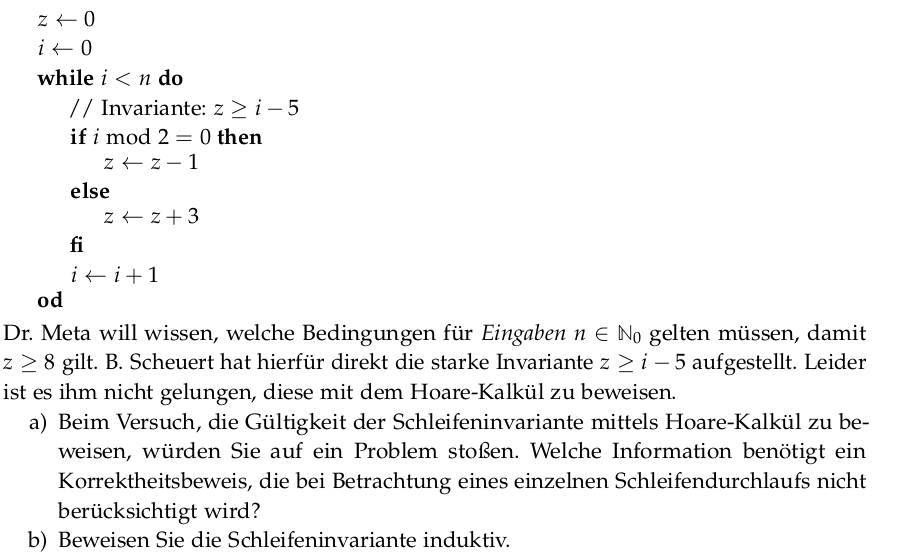
\includegraphics[width=\textwidth,height=\textheight,keepaspectratio]{A12.4_UB2122.png}
\end{frame}

\begin{frame}{Organisation}
	\begin{itemize}
		\item Übungsschein-Anmeldung noch bis 06.März
		\item Klausur-Anmeldung noch bis 06.März
		\item Nur noch \textbf{2 Wochen} bis zur Klausur \impl Spätestens jetzt mit Lernen anfangen
	\end{itemize}
\end{frame}

\framePrevEpisode

\begin{frame}{Kahoot!}
	\begin{itemize}
		\item Heute noch ein paar Fragen aus dem ganzen Semester!
		\item Ihr bekommt Punkte für schnelles und richtiges raten
		\pause
		\item Ich schalte das Quiz frei und ihr könnt über \url{https://kahoot.it} beitreten
		\item Das Kahoot! könnt ihr euch später nochmal unter diesem Link angucken: \\
			\url{https://create.kahoot.it/share/gbi-ubungsstunde/9733f7de-4557-4cba-ad73-c7cb64578e82}
	\end{itemize}
\end{frame}

\section{Wegematrix}

\begin{frame}{Potenzen einer Adjazenzmatrix}
	Bestimmt die Matrix $A^2$ des folgenden Graphen, wobei $A$ die Adjazenzmatrix bezeichne.
	\begin{figure}[H]
		\centering 
		\begin{tikzpicture}[->,>=stealth,baseline=-5mm]
		\matrix[matrix of math nodes,nodes={draw,circle,minimum size=5mm,inner sep=2pt},row sep=10mm,column sep=10mm,ampersand replacement=\&]
		{
			|(0)| 0 \& |(1)| 1 \& |(2)| 2 \& |(3)| 3 \& \\
		};
		\draw  (0) -- (1);
		\draw (1) -- (2);
		\draw (2) -- (3);
		\path (2) edge [loop below] ();
		\end{tikzpicture}
	\end{figure}
	\pause
	$$ A = \begin{pmatrix}
	0 & 1 & 0 & 0 \\ 0 & 0 & 1 & 0 \\ 0 & 0 & 1 & 1 \\ 0 & 0 & 0 & 0
	\end{pmatrix} \qquad \pause A^2 = \begin{pmatrix}
	0 & 0 & 1 & 0 \\ 0 & 0 & 1 & 1 \\ 0 & 0 & 1 & 1 \\ 0 & 0 & 0 & 0 
	\end{pmatrix} $$ \pause
	$(A^2)_{ij}$ gibt also Auskunft, wieviele Pfade der Länge 2 es von $i$ nach $j$ gibt.\\ \pause 
	$(A^n)_{ij}$ allgemein gibt Auskunft, wieviele Pfade der Länge $n$ es von $i$ nach $j$ gibt. 
\end{frame}

\begin{frame}{Wegematrix}
	\begin{Definition}
		Die Wegematrix $W$ ist definiert als $$W_{ij} = \begin{cases} 0 & (i,j) \notin E^\ast \\ 1 & (i,j) \in E^\ast \end{cases} $$
	\end{Definition}

	\pause
	Dabei ist $E^* = \bigcup_{k=0}^{\infty} E^k$ die \textbf{Erreichbarkeitsrelation}, das ist die reflexiv-transitive Hülle der Kantenrelation $E$.\\
	Es ist $(i,j) \elem E^* \Gdw \text{von $i$ aus ist $j$ \textbf{erreichbar}}.$ \\
	\pause
	Die Wegematrix lässt sich daher folgendermaßen berechnen: 
	$$ W = \sgn\left(\summe{k=0}{n-1} A^k \right) $$
	
	\pause
	Warum reicht es hier, in der Summe bis $n-1$ zu gehen?\\ \pause
	Pfade mit einer Länge $\geq n$ enthalten einen Zyklus!
\end{frame}

\begin{frame}{Wegematrix}
	\begin{Beispiel}
		\begin{columns}
			\column{0.4\linewidth}
			\begin{figure}[H]
				\begin{tikzpicture}[->,>=stealth,baseline=-5mm]
				\matrix[matrix of math nodes,nodes={draw,circle,minimum size=5mm,inner sep=2pt},row sep=10mm,column sep=10mm,ampersand replacement=\&]
				{
					|(0)| 0 \& |(1)| 1 \& |(2)| 2 \\
					\& |(3)| 3 \& \\
				};
				\draw  (0) -- (1);
				\draw  (0) -- (3);
				\draw (1) -- (3);
				\draw  (2)  to [bend left] (3);
				\draw  (2) -- (1);
				\draw  (3) to [bend left] (2);
				\draw  (0) to [bend left]  (2);
				\path (2) edge [loop right] ();
				\end{tikzpicture}
			\end{figure}
			\column{0.5\linewidth} \pause
			$$W = \begin{pmatrix}
			1 & 1 & 1 & 1 \\
			0 & 1 & 1 & 1 \\
			0 & 1 & 1 & 1 \\
			0 & 1 & 1 & 1 \\
			\end{pmatrix}$$
		\end{columns}
	\end{Beispiel}
\end{frame}

\begin{frame}{Aufgabe 1}
	Gegeben sei folgender Graph $G$ 
	\begin{figure}[H]
		\begin{tikzpicture}[->,>=stealth,baseline=-5mm]
		\matrix[matrix of math nodes,nodes={draw,circle,minimum size=7mm,inner sep=2pt},row sep=20mm,column sep=20mm,ampersand replacement=\&]
		{
			|(0)| 0 \& |(1)| 1 \\
			|(2)| 2 \& |(3)| 3 \\
		};
		\draw (0) -- (1);
		\draw (0) -- (3);
		\draw (1) -- (2);
		\draw (1) -- (3);
		\draw (2) -- (0);
		\path (1) edge [loop right] ();
		\path (2) edge [loop left] ();
		\end{tikzpicture}
	\end{figure}
	Gebt die Adjazenzliste, die Adjazenzmatrix und die Wegematrix zu diesem Graphen an.
\end{frame}

\begin{frame}{Lösung für Aufgabe 1}
	$$ A = 
	\begin{pmatrix} 
	0 & 1 & 0 & 1 \\ 
	0 & 1 & 1 & 1 \\ 
	1 & 0 & 1 & 0 \\ 
	0 & 0 & 0 & 0 
	\end{pmatrix} $$ 
	\pause 
	
	$$W = 
	\begin{pmatrix} 
	1 & 1 & 1 & 1 \\ 
	1 & 1 & 1 & 1 \\ 
	1 & 1 & 1 & 1 \\ 
	0 & 0 & 0 & 1 
	\end{pmatrix}$$
\end{frame}

%\begin{frame}{Weiterführendes Material}
%	Mehr dazu:
%	GBI Übung 10, WS 15/16
%\end{frame}

\mycomment{ % skip for 2020/2021
\section{Berechnungsmethoden}

\begin{frame}{Wegematrix-Algorithmus}
	Wie rechnet man das aus? \\
	Naiv:
	\begin{align*}
	&W \leftarrow 0 \\ 
	&\mathbf{for}\ i \gets 0\ \mathbf{to}\ n-1\ \mathbf{do} & \text{// $n$-mal...}  \\
	&\qquad M \gets I \qqquad (I = A^0) \\
	&\qquad\mathbf{for}\ j \gets 1\ \mathbf{to}\ i\ \mathbf{do} & \text{// $i$-mal...} \\
	&\qquad\qquad M \gets M \* A & \text{// $n^2 \* (n + n-1)$ Operationen} \\
	&\qquad\mathbf{od} \\
	&\qquad W \gets W + M & \text{// $n^2$ Operationen} \\
	&\mathbf{od} \\
	&W \gets \sgn(W) &  \text{// $n^2$ Operationen} \\
	\end{align*}
\end{frame}

\begin{frame}{Laufzeit der Berechnung}
	\begin{itemize}[<+->]
		\item Jede Matrix hat $n^2$ Einträge, also ergibt sich für die Summe von $n$ Matrizen $n\cdot n^2=n^3$ Summenoperationen 
		\item  Es gibt $\summe{i=0}{n-1} i = \frac{n(n-1)}{2} $ Matrixmultiplikationen. (Im Algorithmus wird \emph{kein} Speicherplatz für $A^i$ reserviert. Würde bei großen $n$ sehr schnell die Speicherkapazitäten übersteigen.) 
		\item $(B\cdot C)_{ij} = \summe{k=0}{n-1} B_{ik} C_{kj}$, also pro Eintrag einer Matrixmultiplikation, die $n^2$ Einträge hat, $n$ Multiplikationen und $n-1$ Additionen. 
		\item $n^2$ Berechnungen der Signum-Funktion 
	\end{itemize}
	\pause
	Insgesamt also $$ n^2 + n^3 + n^2(n+n-1)\cdot \frac{n(n-1)}{2} = n^5 - \frac{3}{2} n^4 + \frac{3}{2} n^3 + n^2 $$
	Wir betrachten im Allgemeinen nur die führende Ordnung, also $n^5$
\end{frame}

\begin{frame}{Optimierungen}
	Can we do better? \pause
	\bigskip
	
	Betrachten wir nun die Relation $ F = (Id \cup E) $ für eine Kantenmenge $E$. \\  \pause 
	So folgt $$ F^2 = (Id \cup E) \circ (Id \cup E) = Id \cup E \cup E^2 $$ \pause
	Analog : $$ F^4 = (F^2)^2 = (Id\cup E \cup E^2) \circ (Id\cup E\cup E^2) = Id \cup E \cup E^2 \cup E^3 \cup E^4 $$ \pause 
	Also folgt $$ F^{2^m} = \bigcup\limits_{i=0}^{2^m} E^i$$ \\
	Setze $m := \lceil \log_2 n \rceil $.
\end{frame}

\begin{frame}{Optimierungen}
	Can we do better? --- Matrixversion \pause
	\bigskip
	
	Betrachten wir nun $ F = (I + A) $ für eine Adjazenzmatrix $A$. \\  \pause 
	So folgt $$ F^2 = (I + A) \* (I + A) = I + A + A^2 $$ \pause
	Analog : $$ F^4 = \left(F^2\right)^2 = (I + A + A^2) \* (I + A + A^2) = I + A + A^2 + A^3 + A^4 $$ \pause 
	Also folgt $$ F^{2^m} = \sum\limits_{i=0}^{2^m} A^i$$ \\
	Setze $m := \lceil \log_2 n \rceil $. \pause \impl $W = \sgn\big(F^{2^m}\big)$.
\end{frame}

\begin{frame}
	Der Algorithmus sieht nun also folgendermaßen aus 
	\begin{align*}
		&F \leftarrow A + I & \text{// $n^2$} \\ 
		&m \leftarrow \lceil \log_2 n \rceil \\
		&\mathbf{for}\ i \leftarrow 1\ \mathbf{to} \ m \ \mathbf{do} & \text{// $\lceil \log_2 n \rceil$-mal} \\
		&\hspace*{2em} F \leftarrow F \cdot F & \text{// $(n+n-1)\cdot n^2$} \\
		&\mathbf{od}\\
		& W\leftarrow \sgn(F) 	& \text{// $n^2$}
	\end{align*} \pause
	Wir brauchen also nur noch $n^2 + \lceil \log_2 n \rceil \left( (2n-1)\cdot n^2 \right) +n^2 = \lceil \log_2 n \rceil \cdot 2n^3 + \dots $ Rechenoperationen  \\
\end{frame}

\begin{frame}{Der Warshall-Algorithmus}
	(Noch) schnellere Berechnung der Wegematrix. Laufzeit $O(n^3)$\\
	Mehr dazu in der Vorlesung und im Skript.
	% TODO: Evtl. doch noch anreißen, evtl. zumindest Folie dazu...
	% ^ Sicher? Ist das nötig?
\end{frame}

}

\begin{frame}{Weitere Graphenprobleme}
	\begin{itemize}[<+->]
		\item Kürzeste Wege
		\item Minimale Spannbäume
		\item (Starke) Zusammenhangskomponenten
		\item Minimale Tour (TSP, „Travelling Salesman Problem“)
	\end{itemize}
	\thasse{
	\pause
	\begin{figure}[H]
		\centering
		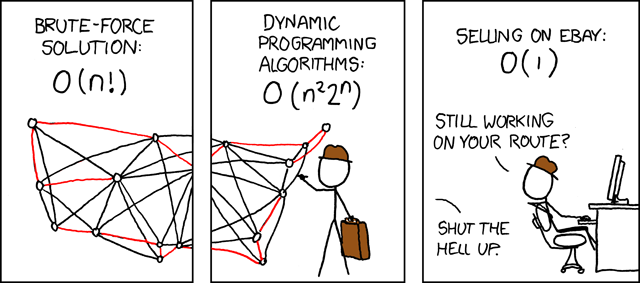
\includegraphics[scale=0.5]{xkcd/tsp_399}
		\caption{ \texttt{\url{http://www.xkcd.com/399}} }
	\end{figure} 	
	}
	

\end{frame}

%\subsection{Warshall-Algorithmus}
%\begin{frame}
%	\only<1>{Schneller geht es mit dem Warshall-Algorithmus!}
%	\only<2>{\begin{align*}
%		&\mathbf{for}\ i\leftarrow 0 \ \mathbf{to} \ n-1 \ \mathbf{do}  \\
%		&\hspace*{2em} \mathbf{for}\ j \leftarrow 0 \ \mathbf{to} \ n-1 \ \mathbf{do} \\
%		& \hspace*{4em} W_{ij} \leftarrow \begin{cases} 1 & i = j \\ A_{ij} & i\neq j \end{cases}  \\
%		&\hspace*{2em} \mathbf{od} \\
%		& \mathbf{od} \\
%		& \mathbf{for}\ k \leftarrow 0 \ \mathbf{to} \ n-1\ \mathbf{do} \\
%		& \hspace*{2em} \mathbf{for}\ i\leftarrow 0 \ \mathbf{to} \ n-1 \ \mathbf{do} \\
%		& \hspace*{4em} \mathbf{for}\ j\leftarrow 0 \ \mathbf{to}\ n-1 \ \mathbf{do} \\
%		& \hspace*{6em} W_{ij} \leftarrow \max\left( W_{ij} , \min(W_{ik},W_{kj}) \right) \\
%		& \hspace*{4em} \mathbf{od}\\
%		& \hspace*{2em} \mathbf{od} \\
%		& \mathbf{od} 	
%		\end{align*}}
%	\only<3>{\begin{align*}
%		&\mathbf{for}\ i\leftarrow 0 \ \mathbf{to} \ n-1 \ \mathbf{do} & // n  \\
%		&\hspace*{2em} \mathbf{for}\ j \leftarrow 0 \ \mathbf{to} \ n-1 \ \mathbf{do} & // n \\
%		& \hspace*{4em} W_{ij} \leftarrow \begin{cases} 1 & i = j \\ A_{ij} & i\neq j \end{cases} & // 1 \\
%		&\hspace*{2em} \mathbf{od} \\
%		& \mathbf{od} \\
%		& \mathbf{for}\ k \leftarrow 0 \ \mathbf{to} \ n-1\ \mathbf{do} & // n \\
%		& \hspace*{2em} \mathbf{for}\ i\leftarrow 0 \ \mathbf{to} \ n-1 \ \mathbf{do} & // n \\
%		& \hspace*{4em} \mathbf{for}\ j\leftarrow 0 \ \mathbf{to}\ n-1 \ \mathbf{do} & // n \\
%		& \hspace*{6em} W_{ij} \leftarrow \max\left( W_{ij} , \min(W_{ik},W_{kj}) \right) & // 1 \\
%		& \hspace*{4em} \mathbf{od}\\
%		& \hspace*{2em} \mathbf{od} \\
%		& \mathbf{od} 	
%		\end{align*}}
%\end{frame}
%
%\begin{frame}
%	\frametitle{Der Warshall-Algorithmus}
%	Da wir hier binäre Werte haben, gilt: $$ \max\left( W_{ij} , \min(W_{ik},W_{kj}) \right) = W_{ij} \vee \left( W_{ik} \wedge W_{kj} \right) $$ \pause 
%	Es ergibt sich insgesamt also eine Laufzeit von $$ n^3+n^2$$ 
%\end{frame}
%
%\begin{frame}
%	\frametitle{Der Warshall-Algorithmus}
%	Was sagt die Matrix $W$ an der Stelle $W_{ij}$ nach dem $k-ten$ Durchlauf im Warshall-Algorithmus aus? \\ \pause
%	Stimmt dieser Algorithmus eigentlich?
%\end{frame}
%
%\begin{frame}
%	\frametitle{Warshall beweisen}
%	\begin{block}{Schleifeninvariante}
%		Für alle $i,j\in \G_n \wedge i\neq j$ gilt : Nach $k$ Durchläufen hat die Matrix den Wert $1$ an der Stelle ($i,j$), genau dann wenn es einen wiederholungsfreien Pfad von $i$ nach $j$ über Knoten in $\G_k$ gibt. Bei $i=j$ steht dort eine $1$. \\
%	\end{block}	
%	
%	\pause
%	Beweis auf Seite 117 im GBI-Skript von Herr Worsch. 
%\end{frame}


%\subsection{Aufgabe 2}
%\begin{frame}
%	\frametitle{Aufgabe 2}
%	Gegeben sei folgende Adjazenzmatrix $$ A = \begin{pmatrix}
%	0 & 1 & 0 & 1 & 1 \\ 0 & 1 & 0 & 1 & 0 \\ 1 & 1 & 0 & 1 & 1 \\ 1 & 1 & 1 & 0 & 1 \\ 0 & 0 & 0 & 0 & 0 
%	\end{pmatrix} $$ 
%	Zeichnen Sie den dazugehörigen Graphen und geben Sie die Initialisierungsmatrix sowie alle Zwischenmatrizen beim Warshall-Algorithmus an. 
%\end{frame}
%
%\subsection{Lösung zu Aufgabe 2}
%\begin{frame}
%	\begin{figure}[H]
%		\begin{tikzpicture}[->,>=stealth,baseline=-5mm]
%		\matrix[matrix of math nodes,nodes={draw,circle,minimum size=9mm,inner sep=2pt},row sep=10mm,column sep=10mm,ampersand replacement=\&]
%		{
%			|(0)| 0 \& \& |(1)| 1 \\
%			\& |(3)| 3 \\
%			|(2)| 2 \& \& |(4)| 4 \\
%		};
%		\draw (0) -- (1);
%		\draw (0) to [bend right] (3);
%		\draw (0) to [bend right] (4) ;
%		\path (1) edge [loop right] ();
%		\draw (1) to [bend right] (3);
%		\draw (2) -- (0);
%		\draw (2) to [bend left] (1);
%		\draw (2) -- (4);
%		\draw (3) to [bend right] (0);
%		\draw (3) to [bend right] (1);
%		\draw (3) -- (2);
%		\draw (3) -- (4);
%		\end{tikzpicture}
%	\end{figure}
%\end{frame}
%
%\begin{frame}
%	$$ W_I = \begin{pmatrix}
%	1 & 1&0&1&1\\0&1&0&1&0\\1&1&1&1&1\\1 & 1 & 1 &1 &1 \\ 0 & 0 & 0 & 0 & 1 
%	\end{pmatrix} $$ \pause
%	$$ W_0 = W_I = W_1 = W_2 $$ \pause
%	$$ W_3 = \begin{pmatrix}
%	1 & 1 & 1 & 1 & 1 \\ 1 & 1 & 1 & 1 & 1 \\ 1 & 1 & 1 & 1 & 1 \\ 1 & 1 & 1 & 1 & 1 \\ 0 & 0 & 0 & 0 & 1 
%	\end{pmatrix} $$ \pause
%	$$ W_4 = W_3 = W$$ 
%\end{frame}

\section{Halbordnungen}
\subsection{Definition}
\begin{frame}
	\begin{Definition}
		Eine Relation $R\subseteq M\times M$ heißt \emph{antisymmetrisch}, wenn für alle $x,y\in M$ gilt $$ xRy \wedge yRx \implies x=y $$
	\end{Definition}
	\pause
	
	\begin{Definition}
		Eine Relation $R\subseteq M\times M$ heißt \emph{Halbordnung}, wenn sie 
		\begin{itemize}
			\item reflexiv
			\item antisymmetrisch
			\item transitiv 
		\end{itemize}
		ist. 
	\end{Definition}

\end{frame}

\subsection{Beispiel}
\begin{frame}
	\emph{Beispiel:} Sei $\sqsubseteq_p$ derart, dass für $v,w\in A^\ast$ gilt: $$ v \sqsubseteq_p w \iff \exists u\in A^\ast : vu = w $$ \pause
	\only<2-3>{Was sagt diese Halbordnung aus? \pause $v\sqsubseteq_p w$ heißt , dass $v$ ein Präfix von $w$ ist. \pause }
	\emph{Beweis}
	\only<4-6>{\begin{itemize}
		\only<4>{\item \emph{Reflexivität}
			$$ v \sqsubseteq_p v \iff \exists u\in A^\ast : vu = v \implies u = \varepsilon $$ Dies ist möglich, da $\varepsilon \in A^\ast$ }
		\only<5>{\item \emph{Antisymmetrie} \begin{align*}
			v\sqsubseteq_p w \wedge w\sqsubseteq_p v &\iff \exists u\in A^\ast : vu = w \wedge \exists \kappa\in A^\ast : w\kappa = v \\ &\implies w\kappa u = w \\ &\implies \kappa = u = \varepsilon \\ &\implies v = w 
		\end{align*}
		}
		\only<6>{ \item \emph{Transitivität}
		\begin{align*}
			v\sqsubseteq_p w \wedge w\sqsubseteq_p x &\iff \exists u\in A^\ast : vu = w \wedge \exists \kappa\in A^\ast : w\kappa = x \\ &\implies vu\kappa = x \\ &\overset{\alpha=u\kappa}{\iff} \exists \alpha\in A^\ast: v\alpha = x \\ &\iff v\sqsubseteq_p x
		\end{align*}
		 }
	\end{itemize}}
\end{frame}

\subsection{Aufgaben}
\begin{frame}
	Zeigen Sie, dass $\leq $ und $\subseteq$ Halbordnungen sind.
\end{frame}
\subsection{Lösung}
\begin{frame}
	Betrachte die Relation $\leq$. Dann gilt mit $$ a\leq b \iff \exists \alpha \in \R^+_0 : a + \alpha = b $$  \pause
	\only<2-4>{
	\begin{itemize}
		\only<2>{\item \emph{Reflexivität}
		\begin{align*}
			a\leq a & \iff \exists \alpha\geq 0 : a + \alpha = a \\ &\implies \alpha = 0 \in \R^+_0
		\end{align*}
		}
		\only<3>{\item
		\emph{Antisymmetrie}
		\begin{align*}
			a \leq b \wedge b \leq a &\iff \exists \alpha, \beta \in\R^+_0 : a + \alpha = b \wedge b + \beta = a \\ &\implies a + \alpha + \beta = a \\ &\overset{\alpha,\beta\geq 0}{\implies} \alpha = \beta = 0 \\ &\implies a = b
		\end{align*}
		}
		\only<4>{\item
		\emph{Transitivität}
		\begin{align*}
			a \leq b \wedge b \leq c &\iff \exists \alpha,\beta \in\R^+_0 : a + \alpha = b \wedge b+\beta = c \\ &\implies a + \alpha + \beta = c \\ &\overset{\gamma=\alpha+\beta}{\implies} \exists \gamma \in\R^+_0 : a + \gamma = c \\ &\implies a\leq c
		\end{align*}
		}
	\end{itemize}	
	}
\end{frame}

\begin{frame}
	Betrachte die Relation $\subseteq$. Dann gilt \pause
	\only<2-9>{
	\begin{itemize}
		\only<2-3>{\item \emph{Reflexivität}
		\begin{align*}
			\only<2>{A \subseteq A &\iff \left( A\subset A \right) \vee \left( A = A \right)}
			\only<3>{A \subseteq A &\iff \left(\textcolor{red}{A\subset A}\right) \vee \left(\textcolor{green}{A = A}\right)}
		\end{align*}
		\only<3>{Dies ist eine wahre Aussage.}
		}
		\only<4-8>{\item
		\emph{Antisymmetrie}
		\begin{align*}
			\only<4-8>{
			A\subseteq B \wedge B\subseteq A \Leftrightarrow & \left( A \subset B \vee A = B \right) \wedge \left( B\subset A \vee B = A \right)
		}
		 \only<5-8>{\\ \Leftrightarrow &  \left( (A\subset B) \wedge \left( B\subset A \vee B = A \right)\right) \\
		 &\vee \left((A = B) \wedge \left( B\subset A \vee B = A \right) \right) \\} 
		\only<6>{\Leftrightarrow &   \left((A\subset B)\wedge (B\subset A) \right) \vee \left( (A\subset B) \wedge (B=A) \right)   \\
		 & \vee  \left( (A=B)\wedge (B\subset A) \right) \vee \left( (A=B) \wedge (B=A) \right)  } 
		\only<7-8>{\Leftrightarrow &   \textcolor{red}{\left((A\subset B)\wedge (B\subset A) \right)} \vee \textcolor{red}{\left( (A\subset B) \wedge (B=A) \right)}   \\
		 & \vee  \textcolor{red}{\left( (A=B)\wedge (B\subset A) \right)} \vee \textcolor{green}{\left( (A=B) \wedge (B=A) \right)}
		 }
		\end{align*}
		}
		\only<8>{Also folgt $$ A\subseteq B \wedge B\subseteq A \implies A = B $$ Dies benutzen wir um Mengengleichheit zu zeigen.
		}
		\only<9>{
		\item
		\emph{Transitivität} 
		\begin{align*}
			A\subseteq B \wedge B\subseteq C &\iff \forall a\in A : a\in B \wedge \forall b\in B : b\in C \\ &\implies a \in C \\ &\implies A\subseteq C
		\end{align*}
		}
	\end{itemize}	
	}
\end{frame}

\subsection{Potenzmengen}
\begin{frame}
	\begin{Definition}
		Als \emph{Potenzmenge} $\mathcal{P}(X)$ ist die Menge aller Teilmengen von $X$ ist definiert. $$ \mathcal{P}(X) = \{ U | U\subseteq X\} $$
		Weitere Notation : $ \mathcal{P}(X) = 2^X $ \\
		
		Für die Mächtigkeit finden wir $$ \vert \mathcal{P}(X) \vert = 2^{\vert X \vert} $$
	\end{Definition} 
	\pause 
	\emph{Beispiel}
	$$ \mathcal{P}(\{a,b\}) = \{ \emptyset, \{a\}, \{b\}, \{a,b\} \} $$
	\pause
	$$\mathcal{P}(\{a,b,c\}) = \{ \emptyset, \{a\}, \{b\}, \{c\}, \{a,b\}, \{a,c\}, \{b,c\}, \{a,b,c\} \} $$
\end{frame}

\begin{frame}
	Betrachten wir nun die Halbordnung $\subseteq$ auf der Menge $\mathcal{P}(\{a,b,c\})$ \pause
	\begin{figure}[H]
		\centering
		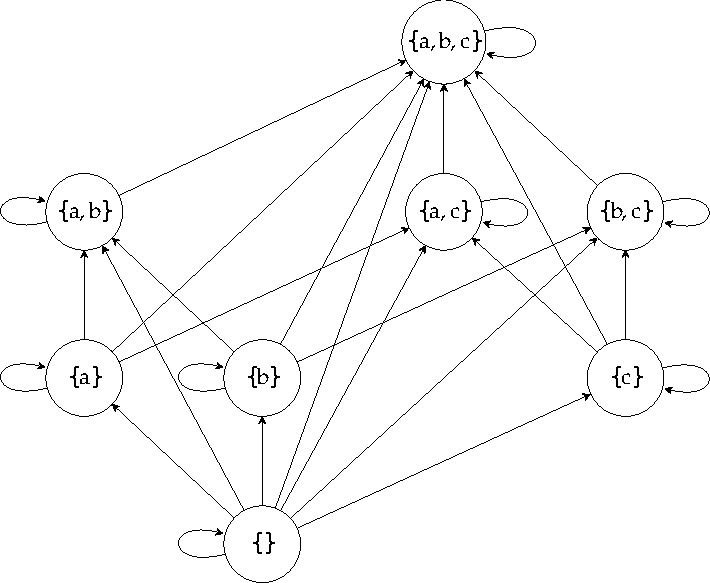
\includegraphics[scale=0.7]{../figures/halbordnungen/Halbordnung.pdf}
	\end{figure} \pause
	Wird doch recht bald unübersichtlich!
\end{frame}

\section{Hasse-Diagramm}
\begin{frame}
Lassen wir nun einfach die Kanten weg, die sich durch Transitivität und Reflexivität ergeben \pause
\begin{figure}[H]
	\centering
	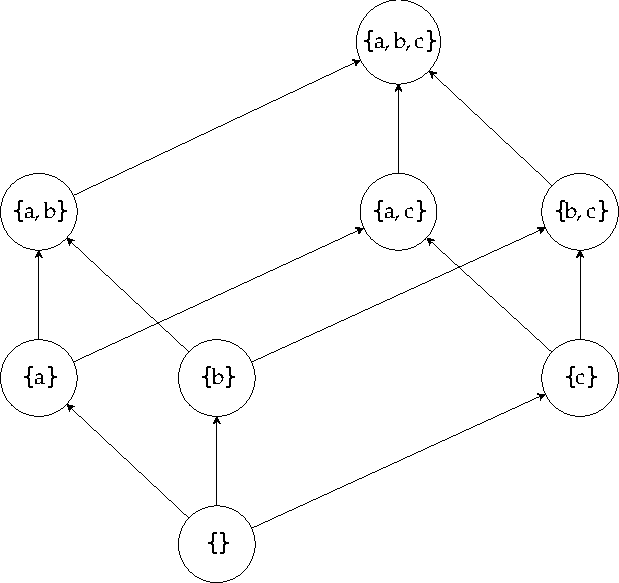
\includegraphics[scale=0.65]{../figures/halbordnungen/Hasse1.pdf}
\end{figure} \pause
Dies nennen wir das \emph{Hasse-Diagramm}.
\end{frame}

\subsection{Definition}
\begin{frame}
	\begin{Definition}
		Eine Diagramm einer Halbordnung $\sqsubseteq$ auf einer Menge $M$ heißt \emph{Hasse-Diagramm}, wenn es im Diagramm eine Kante gibt von $a$ nach $b$, $a,b\in M$, sofern gilt $$ \nexists c\in M : a\sqsubseteq c \sqsubseteq b $$
	\end{Definition} \pause
	
	\begin{Definition}
		Es sei $(M,\sqsubseteq)$ eine halbgeordnete Menge und $T\subseteq M$. Ein Element $x\in T$ heißt 
		\begin{itemize}
			\item \emph{minimales Element} von $T$, wenn es kein $y\in T, y\neq x$ gibt, mit $y\sqsubseteq x$.
			\item \emph{maximales Element} von $T$, wenn es kein $y\in T, y\neq x$ gibt, mit $x\sqsubseteq y$.
			\item \emph{größtes Element} von $T$, wenn für alle $y\in T$ gilt $y\sqsubseteq x$
			\item \emph{kleinstes Element} von $T$, wenn für alle $y\in T$ gilt $x\sqsubseteq y$
		\end{itemize}
	
	\end{Definition}
\end{frame}

%\begin{frame}
%	Beispiele an der Tafel zu $\sqsubseteq = \subseteq$ und $ M \in \{ \mathcal{P}(\{a\}), \mathcal{P}(\{a\})\cup \{d\}, \{a\}\cup\{d\} \}$
%\end{frame}



\subsection{Aufgabe}
\begin{frame}{WS 10/11}
	Geben Sie das Hasse-Diagramm einer Halbordnung auf einer dreielementigen Menge an, die genau zwei maximale und zwei minimale Elemente besitzt.
\end{frame}
\subsection{Lösung}
\begin{frame}
	\begin{figure}[H]
		\centering
		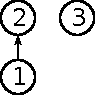
\includegraphics[scale=0.7]{../figures/halbordnungen/Loesung.pdf}
	\end{figure}
\end{frame} %maybe not lets see

\section{Aufgaben}
\begin{frame}{Aufgabe 1: Sprachen}
	\begin{block}{Aufgabe}
		Gegeben seien die folgenden Sprachen:
		\begin{itemize}
			\item[] $L_1 = \left\{\word a^n\word b^m \quad \middle| \quad n,m\in\mathbb{N}_0, n>m\right\}$
			\item[] $L_2 = \left\{\word a^n \word b^m \word c^o \quad \middle| \quad n,o\in\mathbb{N}_0, m\in\mathbb{N}_+\right\}$
		\end{itemize}
		\begin{itemize}
			\item[a)] Geben Sie für $i\in\left\{1,2\right\}$ einen regulären Ausdruck $R_i$ an, sodass gilt: $\lang{R_i}=L_i$. \\
				Falls eine der Sprachen nicht regulär ist, geben Sie eine kontextfreie Grammatik an, die diese Sprache erzeugt.
			\item[b)] Geben Sie für jede reguläre Sprache $L_i$ ($i\in\left\{1,2\right\}$) einen endlichen Akzeptor $A_i$ an, der genau $L_i$ akzeptiert.
		\end{itemize}
	\end{block}
\end{frame}

\begin{frame}{Aufgabe 1: Sprachen}
	\begin{block}{Lösung a)}
		\begin{itemize}
			\item $G_1=(\{S,X\},\{\word{a}, \word{b}\},S, \{S \rightarrow \word{a}S\word{b}|X, X \rightarrow \word{a}X|\word{a}\})$
			\item $R_2=\word{a}\ast\word{b}\word{b}\ast\word{c}\ast$
		\end{itemize}
	\end{block}
	\begin{block}{Lösung b)}
		\begin{center}
			\begin{tikzpicture}[->,>=stealth,shorten >=1pt,auto,node distance=15mm,
			semithick,initial text={}]
			\tikzstyle{every state}=[]
			
			\node[initial,state] (A)                    {$a$};
			\node[state,accepting] (B)  [right of=A]     {$b$};
			\node[state,accepting]		 (M)  [right of=B]		{$c$};
			\node[state]		 (F)  [below of=B]		{$f$};
			
			\path
			(A) edge [loop above]  node {\word a} (A) 
			(A) edge 			  node {\word b} (B) 
			(A) edge 			  node {\word c} (F) 
			(B) edge [loop above]  node {\word b} (B) 
			(B) edge 			  node {\word c} (M)
			(B) edge 			  node {\word a} (F)
			(M) edge [loop above] node {\word c} (M)
			(M) edge 			  node {\word a, \word b} (F)
			(F) edge [loop below] node {\word a, \word b, \word c} (F);
			\end{tikzpicture}
		\end{center}
	\end{block}
\end{frame}

%% Was ihr nun wissen solltet
\section{Schluss}
\def\abbrsize{\footnotesize}
\begin{frame}
	\begin{block}{Und so geht es weiter...}
		\vspace{-.3\baselineskip}
		\begin{itemize}
			\item \textbf{Algo}{\abbrsize rithmen} \textbf{I} \\  -- Mehr zu Algorithmen, Laufzeiten, Datenstrukturen, Graphen
			\item \textbf{T}{\abbrsize echnische} \textbf{I}{\abbrsize nformatik} \\ -- Realisierung von Schaltungen, Prozessoren (MIMA, ...)
			\item \textbf{T}{\abbrsize heoretische} \textbf{G}{\abbrsize rundlagen der} \textbf{I}{\abbrsize nformatik} \\ -- Mehr zu Grammatiken, Komplexität, Entscheidbarkeit, Turingmaschinen
		\end{itemize}
	\end{block}
\end{frame}

%TODO replacement!!! Old xkcd
{\xkcdframevert{2374}{Viel Erfolg  bei euren Klausuren! \smiley}{2.5}}
%\thasse{\lastframe{0.5}{0}{xkcd/proofs_1724.png}{https://www.xkcd.com/1724/}}

\slideThanks
\end{document}